\documentclass[12pt]{amsart}
\usepackage[fullpage]{geometry}
\usepackage{fullpage}
\usepackage{pbox}
\usepackage{graphicx}
\usepackage{booktabs} % Top and bottom rules for table
\usepackage{amsfonts, amsmath, amsthm, amssymb}
\usepackage{longtable,array,color,xcolor}
\usepackage[colorlinks = true,
            urlcolor  = blue]{hyperref}
\usepackage{verbatim}
\usepackage{enumerate}
\newcommand\narrowstyle{\SetTracking{encoding=*}{-50}\lsstyle}

\setlength{\parindent}{0pt}

\begin{document}

\title{Math 320: Homework 4}
Due: October 14, 2016
\maketitle

Please read through chapters 5 and 6 in the textbook.
Answer the following questions. Please submit all code
and output with brief descriptions of what you are doing.

\vspace{5mm}

\begin{enumerate}

\item Problem 7.7.

Let $f(x) = 4x -  1.8x^2 + 1.2x^3 - 0.3x^4$.
\begin{enumerate}
\item Golden-section search ($x_l = -2, x_u = 4, \epsilon_s = 1\%$).

To implement the golden section search, we use the following code,
which corrects several errors in the textbook's code. It also
saves time by evaluating the function at each new point only once.

\begin{verbatim}
function [x, fx, ea, iter]=goldmin(f,xl,xu,es,maxit,varargin)
%minimizes function f given lower and upper bounds on interval
%a stopping criterion of approximate relative error es,
%and maximum number of iterations maxit
%output: x-value yielding minimum fx, approximate relative 
%error at termination, and number of iterations performed.

phi = (1 + sqrt(5))/2;
iter = 0;
d = (phi - 1)*(xu - xl);
x1 = xl + d; 
x2 = xu - d;
fprintf('x1 = %f, x2 = %f \n', x1,x2);
fx1 = f(x1); fx2 = f(x2);
while(1)
    if fx1 < fx2
        xopt = x1;
        xl = x2;
        x2 = x1; fx2 = fx1;
        d = (phi - 1)*(xu - xl);
        x1 = xl + d; fx1 = f(x1);
    else
        xopt = x2;
        xu = x1;
        x1 = x2; fx1 = fx2;
        d = (phi - 1)*(xu - xl);
        x2 = xu - d; fx2 = f(x2);
    end
    fprintf('x1 = %f, x2 = %f \n', x1,x2);
    iter = iter + 1;
    if xopt ~= 0, ea = abs((xu - xl)/xopt)*100; end
    if ea <= es | iter >= maxit, break, end
end
x = xopt; fx = f(xopt);
end

\end{verbatim}

Then, to apply the function in this particular problem,
we use the code: 
\begin{verbatim}
f = @(x) -(4*x - 1.8*x^2 + 1.2*x^3 - 0.3*x^4);
xl = -2; xu = 4; es = .001;
[a,b,c,d] = goldmin(f,xl,xu,es,100)
\end{verbatim}

The output is: $x = 2.3263, f(x) = -5.8853, \epsilon_a = 9.5016 \times 10^{-4}$, iteration number $= 26$.

\item Parabolic Interpolation ($x_1 = 1.75, x_2 = 2, x_3 = 2.5$, iterations
$= 5$).

We write the following function to optimize using parabolic interpolation:

\begin{verbatim}
function [x, fx]=parbIntrpMin(f,x1,x2,x3,maxit)
%minimizes a function f, given three starting points x1,x2,x3
%and a maximum number of iterations maxit
%output: x-value yielding minimum f(x), and f(x) at x.
iter = 0;
while(iter < maxit)
    fx1 = f(x1); fx2 = f(x2); fx3 = f(x3);
    numer = (x2 - x1)^2*(fx2 - fx3) - (x2 - x3)^2*(fx2 - fx1);
    denom = (x2 - x1)*(fx2 - fx3) - (x2 - x3)*(fx2 - fx1);
    xopt =  x2 - 0.5 * numer/denom;
    fxopt = f(xopt);
    if xopt > x3, x1 = x2; x2 = x3; x3 = xopt;
    else
        if xopt < x1, x3 = x2; x2 = x1; x1 = xopt;
        else
            if (xopt > x2)
                if fxopt < fx2, x1 = x2; x2 = xopt;
                else
                    x3 = xopt;
                end
            else
                if fxopt < fx2, x3 = x2; x2 = xopt;
                else
                    x1 = xopt;
                end
            end
        end
        fprintf('x1 = %f, x2 = %f, x3 = %f \n', x1,x2,x3);
        iter = iter + 1;
end
x = xopt; fx = f(xopt);

end
\end{verbatim}

We implement this function in this problem using
the code:
\begin{verbatim}
f = @(x) -(4*x - 1.8*x^2 + 1.2*x^3 - 0.3*x^4);
[a,b] = parbIntrpMin(f,1.75,2,2.5,5)
\end{verbatim}
\end{enumerate}

The output is $x = 2.3264$, $f(x) = -5.8853$.

\vfill
\pagebreak

\item Problem 7.37
The situation can be described by the following
picture:
\begin{figure}[h!]
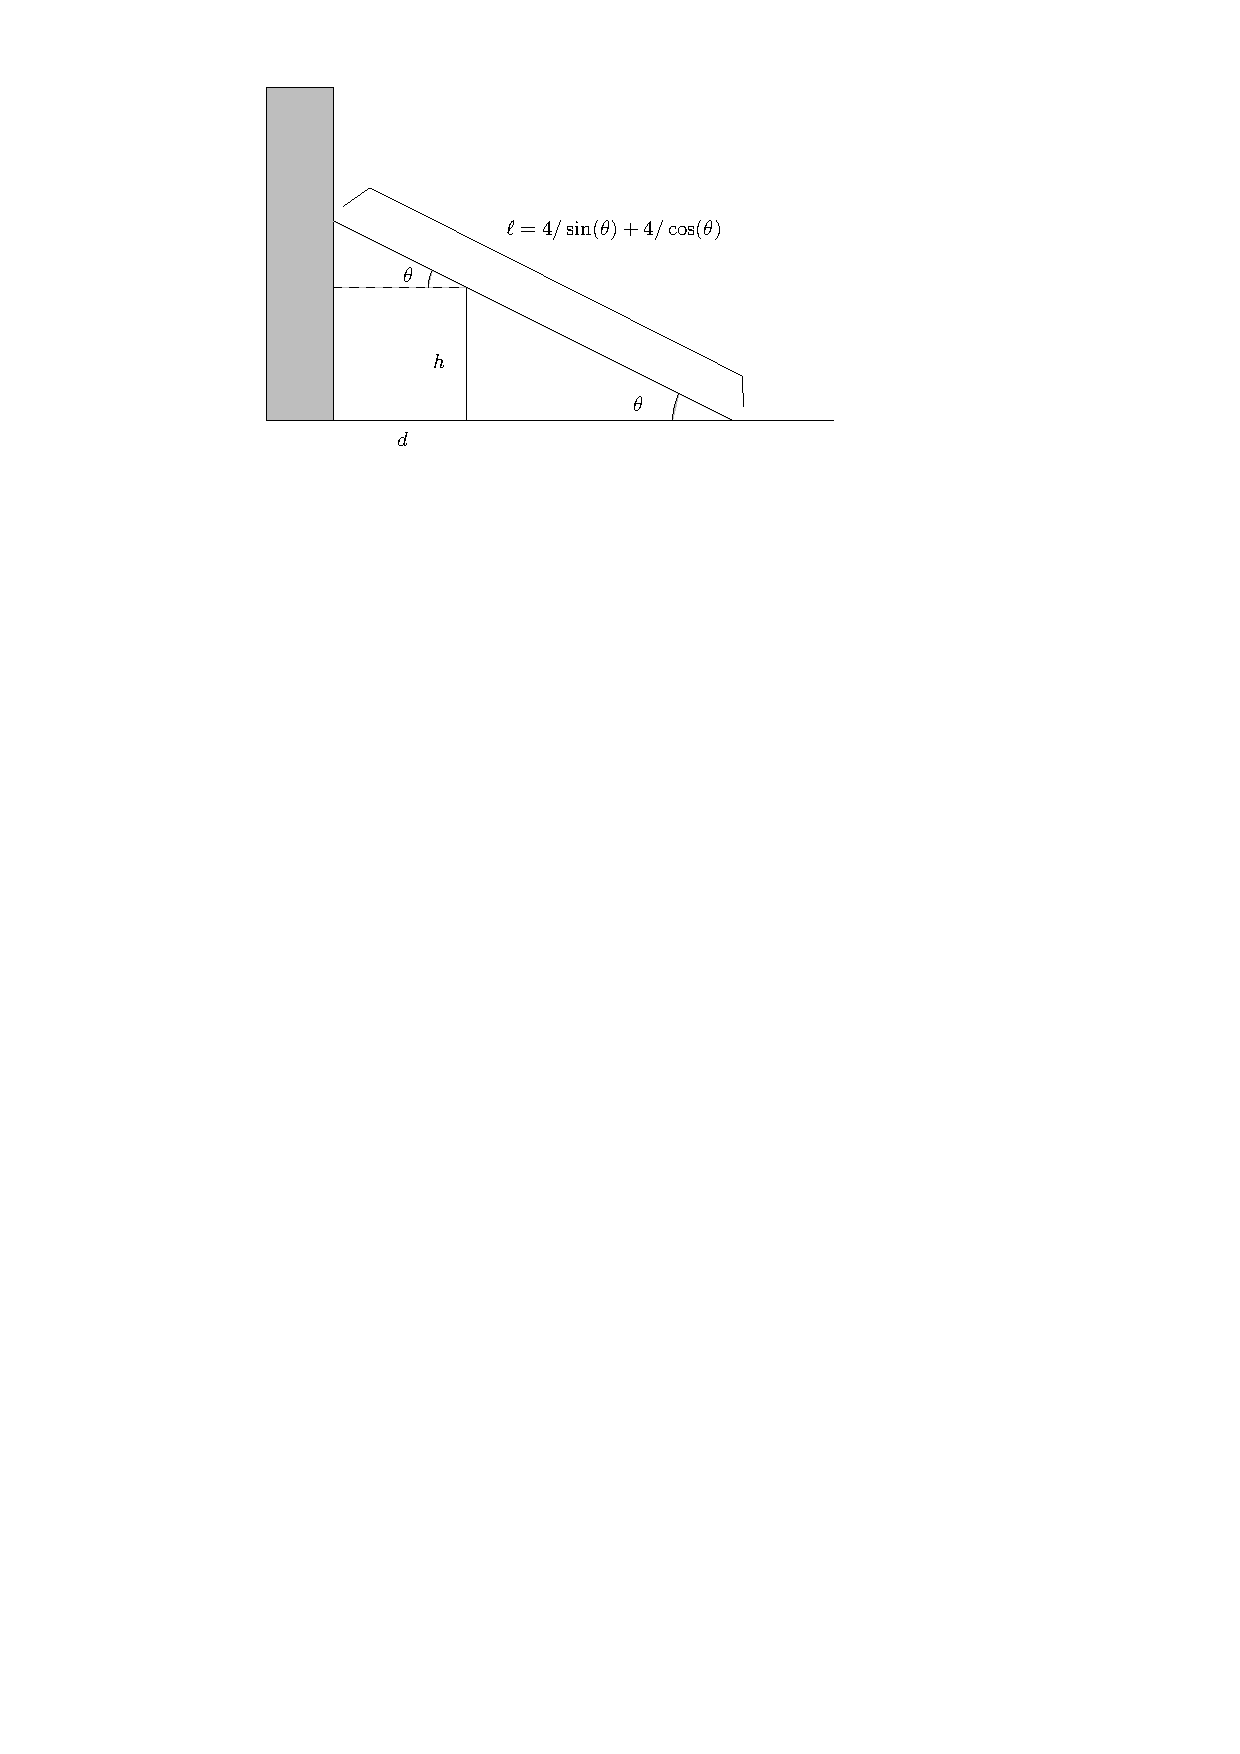
\includegraphics[width=.7\textwidth]{ladder1.pdf}
\end{figure}
The length of the ladder is $\ell = h/\sin(\theta) + d/\cos(\theta)$,
which given $h=d=4$ is $\ell = 4/\sin(\theta) + 4/\cos(\theta)$.

We minimize this function (in terms of $\theta$)
in MATLAB using the following code. We start at
the point $\theta = 1$, since we want $0\leq \theta \leq pi/2 \approx 1.6$.

\begin{verbatim}
f = @(x,h,d) h/sin(x) + d/cos(x);
h = 4; d = 4;
X = fminsearch(@(x) f(x,h,d),1)
\end{verbatim}

The output is $X = 0.7854 \approx pi/4$, for which
$\ell = 11.3137$.


\vfill
\pagebreak

\item Problem 8.3. One matrix form of this system of linear
equations is:
\[
\left(
\begin{array}{ccc}
0 & -6  & 5 \\
0 & 2 & 7 \\
-4 & 3 & -7
\end{array}
\right)\left( 
\begin{array}{c} x_1 \\ x_2 \\ x_3 \end{array}
\right)
= \left( 
\begin{array}{c} 50 \\ -30 \\ 50 \end{array}
\right)
\]

In order to compute the solution, we use the following code:
\begin{verbatim}
A = [0,-6,5; 0, 2, 7; -4, 3, -7];
b = [50, -30, 50]';
x = A\b
\end{verbatim}
Furthermore, we can compute the transpose and inverse of the
coefficient matrix using the commands {\tt A', inv(A)}.

The outputs are $x = (-17.0192,-9.6154,-1.5385)^T$.
\[A^T = \left(
\begin{array}{ccc}
0 & 0  & -4 \\
-6 & 2 & 3 \\
5 & 7 & -7
\end{array}
\right), \hspace{1cm}
A^{-1} = \left(
\begin{array}{ccc}
-0.1683 & -0.1298  & -0.2500 \\
-0.1346 & 0.0962 & 0 \\
0.0385 & 0.1154 & 0
\end{array}
\right)
\]


\vfill
\pagebreak

\item Problem 8.9

\[
\begin{array}{ccccccccccccc}
& & Q_{01}c_{01} & + & Q_{31} c_3 & = & Q_{15} c_1 & + & Q_{12} c_1 &  & \\
& & & & Q_{12} c_1 & = & Q_{25} c_2 & + & Q_{24} c_2 & + & Q_{23} c_2 \\
& & Q_{03} c_{03} & + & Q_{23} c_2 & = & Q_{31} c_3 & + & Q_{34} c_3 \\
Q_{24} c_2 & + & Q_{34} c_3 & + & Q_{54} c_5 & = & Q_{44} c_4 \\
& & Q_{15} c_1 & + & Q_{25} c_2 & = & Q_{54} c_5 & + & Q_{55} c_5 \\
\end{array}
\]

Reformulating to translate into a matrix equation:

\[ {\tiny
\begin{array}{ccccccccccccc}
(Q_{15} + Q_{12}) c_1  & +  & & &  - Q_{31}c_{3} &  & & & &  = &  Q_{01} c_{01}\\
Q_{12} c_1 & + & (-Q_{25} - Q_{24} - Q_{23})c_2 & & & & & & & = & 0 \\
 &  & - Q_{23}c_2 & + & (Q_{31} + Q_{34})c_3 & & & & &  = &  Q_{03} c_{03} \\
& & Q_{24} c_2 & + & Q_{34} c_3 & + & (- Q_{44})c_4 & + & Q_{54} c_5 & = & 0 \\
Q_{15} c_1 & + & Q_{25} c_2 & & & & & + & (-Q_{54} - Q_{55}) c_5 & = & 0\\
\end{array}}
\]

And as a matrix equation,
\[{\small \left(
\begin{array}{ccccc}
(Q_{15} + Q_{12})  & 0 &   - Q_{31} & 0  & 0 \\
Q_{12}   & (-Q_{25} - Q_{24} - Q_{23}) & 0 & 0 & 0  \\
0  & - Q_{23}  & (Q_{31} + Q_{34}) & 0 & 0   \\
0 & Q_{24}  & Q_{34}  & - Q_{44}  & Q_{54} \\
Q_{15}  & Q_{25} & 0 & 0 & (-Q_{54} - Q_{55}) \\
\end{array} \right)
\left(
\begin{array}{c}
c_1 \\ c_2 \\ c_3 \\ c_4 \\ c_5
\end{array}
\right) = 
\left( \begin{array}{c}
 Q_{01} c_{01} \\ 0  \\ Q_{03} c_{03} \\ 0 \\ 0
\end{array} \right)}
\]
Then inserting our values for all the $Q$ and $c$ variables, we have:

\[ \left(
\begin{array}{ccccc}
9 & 0 & -3 & 0 & 0 \\
4 & -4 & 0 & 0 & 0 \\
0 & -2 & 9 & 0 & 0 \\
0 & 1 & 6 & -9 & 2 \\
5 & 1 & 0 & 0 & -6 \\
\end{array}
\right)
\left(
\begin{array}{c}
c_1 \\ c_2 \\ c_3 \\ c_4 \\ c_5
\end{array}
\right) = 
\left( \begin{array}{c}
120 \\ 0  \\ 350 \\ 0 \\ 0
\end{array} \right)
\]
\end{enumerate}

The solution is then $(28.4,28.4,45.2,39.6,28.4)$.
\end{document}
